\documentclass[12pt]{article}
\usepackage{graphicx}
\usepackage{listings}
\usepackage{fullpage}
\usepackage{tikz}
\usepackage{enumitem}
\usetikzlibrary{shapes,arrows,calc,automata}
\tikzstyle{bt} = [rectangle, draw, fill=blue!20, 
    text width=4em, text centered, rounded corners, minimum height=2em]

\lstset{ %
language=Java,
basicstyle=\small \ttfamily,commentstyle=\scriptsize\itshape,showstringspaces=false,breaklines=true,numbers=left}

\usepackage{fontspec}
\setmonofont{Cousine}[Scale=MatchLowercase]

\begin{document}

\title{Software Testing, Quality Assurance \& Maintenance (ECE453/CS447/SE465): Midterm}
\author{}
\renewcommand{\today}{}
\maketitle

 ~\\[-7em]

\begin{center}
{\Large February 17, 2017}
\end{center}

This open-book midterm has 5 questions and 80 points. Answer the
questions in your answer book. You may consult any printed material
(books, notes, etc).


\section*{Question 1: Test Design (10 points)}
Sentence: Splitting the test makes it easier to pinpoint the cause of the failure
because of the descriptive test name and because the tests run more quickly.

\begin{lstlisting}[basicstyle=\scriptsize \ttfamily]
  @Test
  public void testStatic() throws Throwable {
    // L3
  }

  @Test
  public void testDeprecated() throws Throwable {
    // L4
  }

  @Test
  public void testReturnTypes() throws Throwable {
    // L5, L6
  }

  @Test
  public void testParameterTypes() throws Throwable {
    // L7
  }

  @Test
  public void testExceptionTypes() throws Throwable {
    // L8
  }
\end{lstlisting}

\newpage
\section*{Question 2: Fuzzing (10 points)}
\begin{lstlisting}
  void naiveComputeAngleTest() {
    Random r = new Random();
    computeAngle(r.nextInt(), r.nextInt(), r.nextInt());
  }
\end{lstlisting}
This is the bottleneck I mentioned in the notes. Most of the time the
execution of the method under test would simply stop at the {\tt
  IllegalArgumentException} and not reach the key {\tt atan2} call. So, no,
{\tt naiveComputeAngleTest} would not give you good insight into what
{\tt computeAngle} does.

For the next part, I asked the TAs to be fairly lenient, especially with
respect to rounding issues. In particular it was OK to assume that the 
{\tt sqrt} was close enough often enough. There are more clever solutions possible.
But I did ask you to never call {\tt computeAngle} with bad args, so you had
to filter that out.
\begin{lstlisting}
  void smartComputeAngleTest() {
    Random r = new Random();
    while (true) {
      int x = r.nextInt(), y = r.nextInt();
      int z = Math.sqrt(x*x + y*y);
      if (z*z == x*x + y*y) {
        computeAngle(x, y, z);
      }
    }
  }
\end{lstlisting}
A more clever solution (thanks Jun!) would be:
\begin{lstlisting}
  void smartComputeAngleTest() {
    Random r = new Random();
    while (true) {
      int a = r.nextInt(), b = r.nextInt();
      computeAngle(a*a, b*b, a*a + b*b + 2*a*b);
    }
  }
\end{lstlisting}

\newpage
\section*{Question 3: Short-circuit evaluation (15 points)}
Whoops. I had 8 nodes. Sorry. Also, there was a missing return, which you might choose to include or not.
\begin{center}
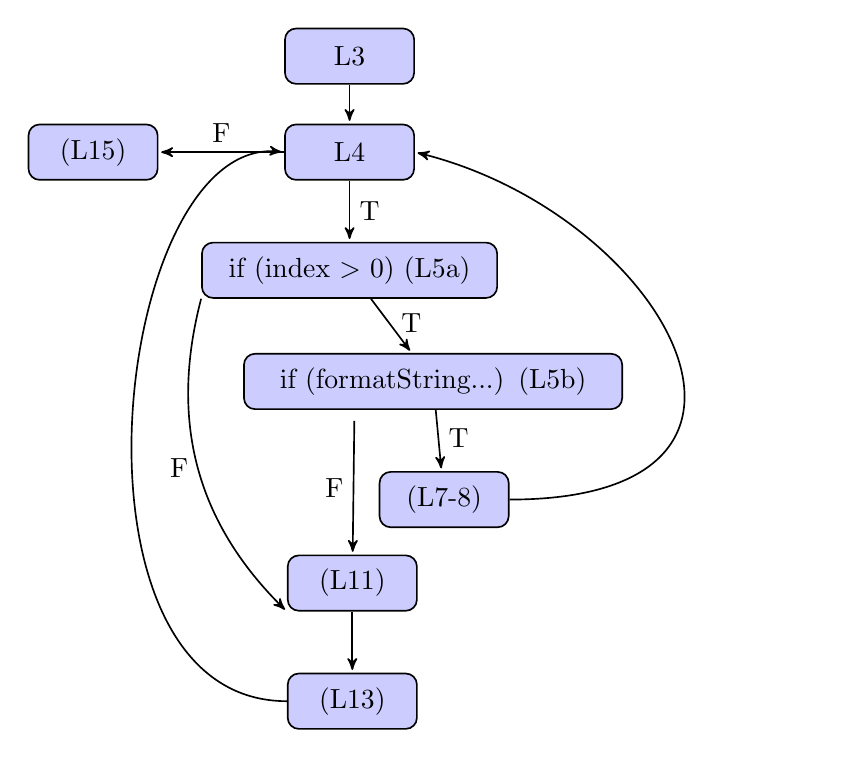
\begin{tikzpicture}[->,>=stealth',shorten >=1pt,auto,node distance=1.5cm,
                    semithick,initial text=]

  \node[bt]           (1) {L3};
  \node[bt]           (2) [below of=1, yshift=.8em] {L4};
  \node[bt,text width=10em]           (3) [below of=2] {if (index $>$ 0) (L5a)};
  \node[bt,text width=13em]           (4) [below right of=3,yshift=-1em] {if (formatString...) (L5b)};
  \node[bt]           (5) [below of=4,xshift=.4em] {(L7-8)};
  \node[bt]           (6) [below left of=5,xshift=-.3em] {(L11)};
  \node[bt]           (7) [below of=6] {(L13)};
  \node[bt]           (8) [left of=2,xshift=-5em] {(L15)};

  \path (1) edge node {} (2)
  (2) edge node {T} (3)
  (2) edge node[above] {F} (8)
  (3) edge node[yshift=-.6em] {T} (4)
  (4) edge node[yshift=-.6em] {T} (5)
  (4) ++ (-1, -.5) edge node[left] {F} (6)
  (3.south west) edge[bend right] node[left] {F} (6.south west)
  (6) edge node {} (7);

  \draw [->] (5.east) .. controls ++ (4, 0) and (4, -2)  .. (2.east);
  \draw [->] (7.west) .. controls ++ (-3, 0) and (-3, -1) .. (2.west);
\end{tikzpicture}
\end{center}

The missing branch is L5a true, L5b false (i.e. 
\verb+(index > 0) && !formatString.charAt(index - 1) == '!'+);
the case \verb+"$"+ is L5a false and done, while the case \verb+"!$"+ is
L5a true, L5b true and done.

The question was somewhat ambiguous about whether the case should achieve 100\%
branch coverage on its own or combined with the two previous test cases.
Due to ambiguity, TAs should accept either one, but it's pretty easy to
make a standalone case that achieves 100\% branch coverage: \verb+"$!$$"+
achieves all of the previous branches and also includes a case where
\verb+formatString.charAt(index - 1) == '!'+.

\newpage
\section*{Question 4: Statement and Branch Coverage (20 points)}
Sorry again. I added a node at the last minute. For reference:
\begin{lstlisting}
public static List<String> wrap(String input, int line_length) {
  List<String> rv = new ArrayList<String>();
  int last_break = -1, last_space = 0;
  
  for (int i = 0;
       i < input.length();
       i++) {
    if (input.charAt(i) == ' ') {
      last_space = i;
    }
    
    if (i - last_break > line_length) {
      rv.add(input.substring(last_break + 1, last_space));
      last_break = i;
    }
  }
  if (last_space >= last_break + 1) {
    rv.add(input.substring(last_break + 1, last_space));
  }
  return rv;
}
\end{lstlisting}

\begin{center}
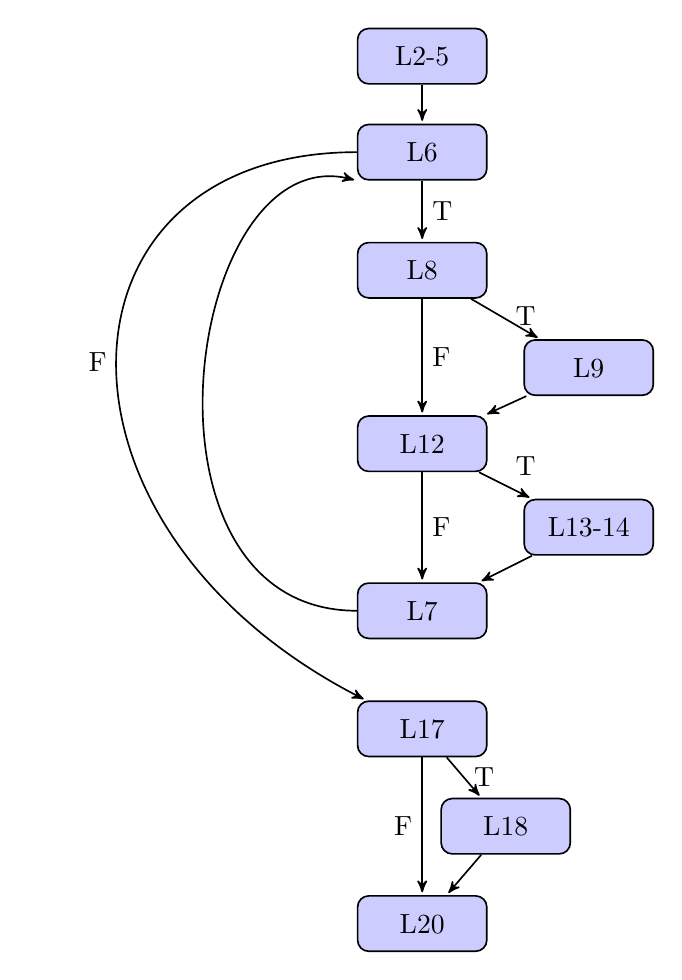
\begin{tikzpicture}[->,>=stealth',shorten >=1pt,auto,node distance=1.5cm,
                    semithick,initial text=]

  \node[bt]           (1) {L2-5};
  \node[bt]           (2) [below of=1, yshift=.8em] {L6};
  \node[bt]           (3) [below of=2] {L8};
  \node[bt]           (4) [below right of=3,xshift=3em,yshift=-.5em] {L9};
  \node[bt]           (5) [below of=3,yshift=-2em] {L12};
  \node[bt]           (6) [below right of=5,xshift=3em] {L13-14};
  \node[bt]           (7) [below left of=6,xshift=-3em] {L7};
  \node[bt]           (8) [below of=7] {L17};
  \node[bt]           (9) [below right of=8,yshift=-.5em] {L18};
  \node[bt]           (10) [below left of=9,yshift=-.5em] {L20};

  \path (1) edge node {} (2)
  (2) edge node {T} (3)
  (3) edge node[yshift=-.6em] {T} (4)
  (3) edge node {F} (5)
  (4) edge node {} (5)
  (5) edge node {T} (6)
  (5) edge node {F} (7)
  (6) edge node {} (7)
  (8) edge node[right] {T} (9)
  (8) edge node[left] {F} (10)
  (9) edge node {} (10);

  \draw [->] (2.west) .. controls ++ (-4, 0) and (-5, -6) .. node[left] {F} (8);
  \draw [->] (7.west) .. controls ++ (-3, 0) and (-3, -1) .. (2.south west);
\end{tikzpicture}
\end{center}


The argument should proceed node-by-node. Lines 2--5 and L6 are obvious enough
that they don't need to be mentioned. Continuing to Line 8, we initially have 
{\tt i = 0} and \verb+input.length > 0+, so we definitely enter the loop.
We also observe that the loop iterates over every possible {\tt i} (it doesn't skip any).
We reach line 9 because the input string contains spaces. Once we're in the loop,
Line 12 is unavoidable. \verb+last_break+ starts at -1 and is only changed inside the
if, and {\tt i - 1} exceeds \verb+line_length+ because we observe more than
one line in the output, so we definitely execute Lines 13--14.
Finally, Line 7 is unavoidable inside the loop as well. Because the program
terminates, we definitely exit the loop and reach Line 17. Finally,
we reach Line 18 because \verb+last_space+ is 13 on exit while \verb+last_break+ is 9.
Line 20 is obvious.

The branches that might not be covered given statement coverage are L8--L12, L12--L7, and L17--L20.
L8--L12 is executed on a non-space input, which the input clearly includes.
L12--L7 also gets executed for characters that don't cause line breaks, which
clearly exists because we observe lines that are longer than 1 letter long.
This input does not execute the branch L17--L20 because we only execute L17 once
and, as we argued above, that execution takes the true branch.

\newpage
\section*{Question 5: Understanding Mutation (25 points)}
For part (a), there are lots of non-trivial mutants. One such mutant is to replace
the constant "1" on line 18 by the constant "0".
This will cause the second line of the output to start with a space.
The mutant is non-trivial: any input which doesn't wrap (e.g. same {\tt input},
\verb+line_length = 40+) does not kill the mutant.

Part (b): Test case \verb+input = "one three two", line_length = 9+ 
without trailing space has the same expected output (\verb+one three\ntwo+)
and actual output \verb+one three+.

Part (c) depends on your answer from part (b).
Another mutant is on Line 17: changing \verb!"+ 1"! to 
\verb!"+ 0"! will cause a crash on my input from (b).
On the other hand, input \verb+input = "one three two ", line_length 9+ shows
that the mutant is non-trivial. (I'd intended a fix for the 
bug but that's actually harder than it seems, especially
without a computer.)

%Part (c): The most obvious mutant is the one that happens to fix the bug (which 
%clearly also kills your test case), but many other mutants are also possible. 
%The fix is on line 14: replace {\tt i} with \verb+last_space+.

\end{document}
